\documentclass{standalone}

\usepackage[OT1]{fontenc}
\renewcommand*\familydefault{\sfdefault}
\usepackage{helvet,sfmath}
\usepackage{siunitx}

\usepackage{tikz}
\usetikzlibrary{arrows,calc,patterns}
% \usetikzlibrary{intersections, calc, arrows.meta}
\usepackage{tikz,tkz-euclide}

\begin{document}



\tikzset{every picture/.style={line width=0.75pt}} %set default line width to 0.75pt        

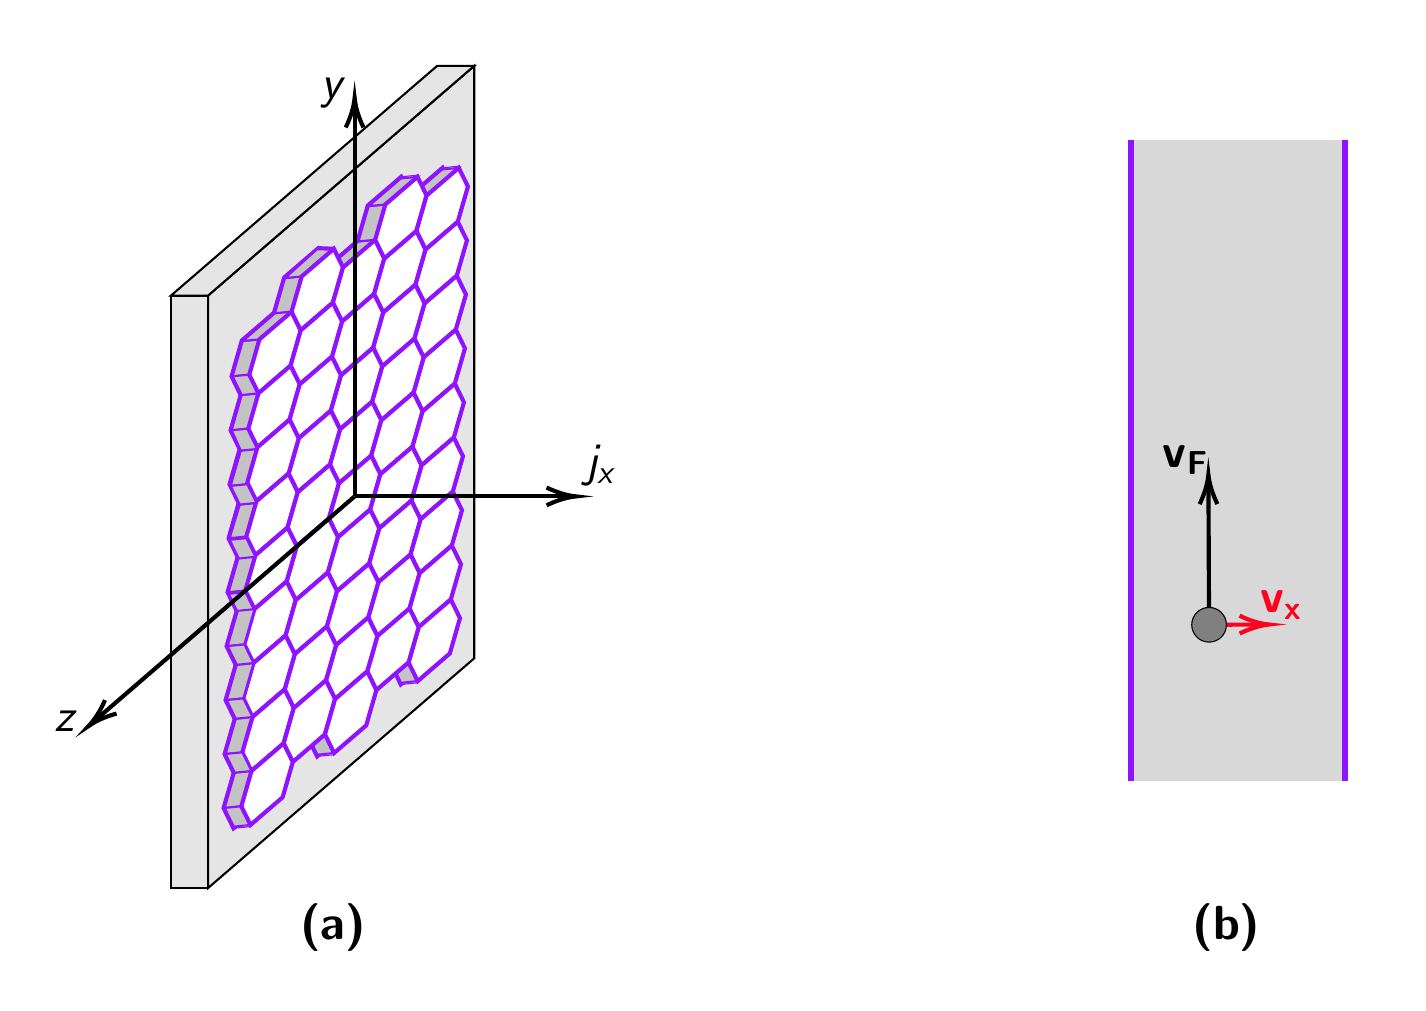
\begin{tikzpicture}[x=0.75pt,y=0.75pt,yscale=-1,xscale=1]
%uncomment if require: \path (0,2520); %set diagram left start at 0, and has height of 2520

%% Background

\draw[draw=none] (40,1050) rectangle (700,1510);

%Shape: Polygon [id:ds37858745979201613] 
\draw  [color={rgb, 255:red, 0; green, 0; blue, 0 }  ,draw opacity=1 ][fill={rgb, 255:red, 229; green, 229; blue, 229 }  ,fill opacity=1 ][line width=0.75]  (255.15,1353.83) -- (126.92,1464.5) -- (126.92,1179.05) -- (255.15,1068.39) -- cycle ;
%Shape: Rectangle [id:dp5698242354930484] 
\draw  [color={rgb, 255:red, 0; green, 0; blue, 0 }  ,draw opacity=1 ][fill={rgb, 255:red, 229; green, 229; blue, 229 }  ,fill opacity=1 ][line width=0.75]  (109.05,1179.05) -- (126.92,1179.05) -- (126.92,1464.5) -- (109.05,1464.5) -- cycle ;
%Shape: Polygon [id:ds02848302864329788] 
\draw  [color={rgb, 255:red, 0; green, 0; blue, 0 }  ,draw opacity=1 ][fill={rgb, 255:red, 229; green, 229; blue, 229 }  ,fill opacity=1 ][line width=0.75]  (126.92,1179.05) -- (109.05,1179.05) -- (237.28,1068.39) -- (255.15,1068.39) -- cycle ;

%Flowchart: Preparation [id:dp6428015125114787] 
\draw  [color={rgb, 255:red, 144; green, 19; blue, 254 }  ,draw opacity=1 ][fill={rgb, 255:red, 255; green, 255; blue, 255 }  ,fill opacity=1 ][line width=2.25]  (138.77,1217.96) -- (143.65,1200.96) -- (159.14,1187.63) -- (163.55,1196.63) -- (158.67,1213.63) -- (143.17,1226.95) -- cycle ;
%Flowchart: Preparation [id:dp7028543507315826] 
\draw  [color={rgb, 255:red, 144; green, 19; blue, 254 }  ,draw opacity=1 ][fill={rgb, 255:red, 255; green, 255; blue, 255 }  ,fill opacity=1 ][line width=2.25]  (178.57,1209.3) -- (183.45,1192.3) -- (198.94,1178.97) -- (203.35,1187.97) -- (198.46,1204.97) -- (182.97,1218.3) -- cycle ;
%Flowchart: Preparation [id:dp33811798781617275] 
\draw  [color={rgb, 255:red, 144; green, 19; blue, 254 }  ,draw opacity=1 ][fill={rgb, 255:red, 255; green, 255; blue, 255 }  ,fill opacity=1 ][line width=2.25]  (159.14,1187.63) -- (164.03,1170.64) -- (179.52,1157.31) -- (183.93,1166.31) -- (179.04,1183.3) -- (163.55,1196.63) -- cycle ;
%Flowchart: Preparation [id:dp6361917591377868] 
\draw  [color={rgb, 255:red, 144; green, 19; blue, 254 }  ,draw opacity=1 ][fill={rgb, 255:red, 255; green, 255; blue, 255 }  ,fill opacity=1 ][line width=2.25]  (179.04,1183.3) -- (183.93,1166.31) -- (199.42,1152.98) -- (203.83,1161.98) -- (198.94,1178.97) -- (183.45,1192.3) -- cycle ;
%Flowchart: Preparation [id:dp08177445863249344] 
\draw  [color={rgb, 255:red, 144; green, 19; blue, 254 }  ,draw opacity=1 ][fill={rgb, 255:red, 255; green, 255; blue, 255 }  ,fill opacity=1 ][line width=2.25]  (158.67,1213.63) -- (163.55,1196.63) -- (179.04,1183.3) -- (183.45,1192.3) -- (178.57,1209.3) -- (163.07,1222.63) -- cycle ;
%Flowchart: Preparation [id:dp4671950049961553] 
\draw  [color={rgb, 255:red, 144; green, 19; blue, 254 }  ,draw opacity=1 ][fill={rgb, 255:red, 255; green, 255; blue, 255 }  ,fill opacity=1 ][line width=2.25]  (198.94,1178.97) -- (203.83,1161.98) -- (219.32,1148.65) -- (223.73,1157.65) -- (218.84,1174.64) -- (203.35,1187.97) -- cycle ;
%Flowchart: Preparation [id:dp30525817597012217] 
\draw  [color={rgb, 255:red, 144; green, 19; blue, 254 }  ,draw opacity=1 ][fill={rgb, 255:red, 255; green, 255; blue, 255 }  ,fill opacity=1 ][line width=2.25]  (199.42,1152.98) -- (204.31,1135.98) -- (219.8,1122.65) -- (224.21,1131.65) -- (219.32,1148.65) -- (203.83,1161.98) -- cycle ;
%Flowchart: Preparation [id:dp34508888512360036] 
\draw  [color={rgb, 255:red, 144; green, 19; blue, 254 }  ,draw opacity=1 ][fill={rgb, 255:red, 255; green, 255; blue, 255 }  ,fill opacity=1 ][line width=2.25]  (219.32,1148.65) -- (224.21,1131.65) -- (239.7,1118.32) -- (244.11,1127.32) -- (239.22,1144.32) -- (223.73,1157.65) -- cycle ;
%Flowchart: Preparation [id:dp828524680067646] 
\draw  [color={rgb, 255:red, 144; green, 19; blue, 254 }  ,draw opacity=1 ][fill={rgb, 255:red, 255; green, 255; blue, 255 }  ,fill opacity=1 ][line width=2.25]  (218.84,1174.64) -- (223.73,1157.65) -- (239.22,1144.32) -- (243.63,1153.32) -- (238.74,1170.31) -- (223.25,1183.64) -- cycle ;
%Flowchart: Preparation [id:dp3138491940146858] 
\draw  [color={rgb, 255:red, 144; green, 19; blue, 254 }  ,draw opacity=1 ][fill={rgb, 255:red, 255; green, 255; blue, 255 }  ,fill opacity=1 ][line width=2.25]  (138.29,1243.95) -- (143.17,1226.95) -- (158.66,1213.63) -- (163.07,1222.62) -- (158.19,1239.62) -- (142.7,1252.95) -- cycle ;
%Flowchart: Preparation [id:dp4068884758377167] 
\draw  [color={rgb, 255:red, 144; green, 19; blue, 254 }  ,draw opacity=1 ][fill={rgb, 255:red, 255; green, 255; blue, 255 }  ,fill opacity=1 ][line width=2.25]  (158.19,1239.62) -- (163.07,1222.62) -- (178.56,1209.3) -- (182.97,1218.29) -- (178.09,1235.29) -- (162.6,1248.62) -- cycle ;
%Flowchart: Preparation [id:dp7451385886830003] 
\draw  [color={rgb, 255:red, 144; green, 19; blue, 254 }  ,draw opacity=1 ][fill={rgb, 255:red, 255; green, 255; blue, 255 }  ,fill opacity=1 ][line width=2.25]  (198.47,1204.97) -- (203.35,1187.97) -- (218.84,1174.64) -- (223.25,1183.64) -- (218.36,1200.64) -- (202.87,1213.97) -- cycle ;
%Flowchart: Preparation [id:dp8877389680893081] 
\draw  [color={rgb, 255:red, 144; green, 19; blue, 254 }  ,draw opacity=1 ][fill={rgb, 255:red, 255; green, 255; blue, 255 }  ,fill opacity=1 ][line width=2.25]  (178.09,1235.29) -- (182.97,1218.29) -- (198.46,1204.97) -- (202.87,1213.97) -- (197.99,1230.96) -- (182.5,1244.29) -- cycle ;
%Flowchart: Preparation [id:dp8921266467695895] 
\draw  [color={rgb, 255:red, 144; green, 19; blue, 254 }  ,draw opacity=1 ][fill={rgb, 255:red, 255; green, 255; blue, 255 }  ,fill opacity=1 ][line width=2.25]  (218.37,1200.64) -- (223.25,1183.64) -- (238.74,1170.31) -- (243.15,1179.31) -- (238.26,1196.31) -- (222.77,1209.64) -- cycle ;
%Flowchart: Preparation [id:dp4632862143796097] 
\draw  [color={rgb, 255:red, 144; green, 19; blue, 254 }  ,draw opacity=1 ][fill={rgb, 255:red, 255; green, 255; blue, 255 }  ,fill opacity=1 ][line width=2.25]  (217.89,1226.63) -- (222.77,1209.64) -- (238.26,1196.31) -- (242.67,1205.31) -- (237.79,1222.3) -- (222.3,1235.63) -- cycle ;
%Flowchart: Preparation [id:dp3973529298148656] 
\draw  [color={rgb, 255:red, 144; green, 19; blue, 254 }  ,draw opacity=1 ][fill={rgb, 255:red, 255; green, 255; blue, 255 }  ,fill opacity=1 ][line width=2.25]  (197.99,1230.96) -- (202.87,1213.97) -- (218.36,1200.64) -- (222.77,1209.64) -- (217.89,1226.63) -- (202.4,1239.96) -- cycle ;
%Flowchart: Preparation [id:dp7895364580872496] 
\draw  [color={rgb, 255:red, 144; green, 19; blue, 254 }  ,draw opacity=1 ][fill={rgb, 255:red, 255; green, 255; blue, 255 }  ,fill opacity=1 ][line width=2.25]  (177.61,1261.29) -- (182.49,1244.29) -- (197.99,1230.96) -- (202.39,1239.96) -- (197.51,1256.96) -- (182.02,1270.28) -- cycle ;
%Flowchart: Preparation [id:dp16728371635810435] 
\draw  [color={rgb, 255:red, 144; green, 19; blue, 254 }  ,draw opacity=1 ][fill={rgb, 255:red, 255; green, 255; blue, 255 }  ,fill opacity=1 ][line width=2.25]  (197.51,1256.96) -- (202.39,1239.96) -- (217.89,1226.63) -- (222.29,1235.63) -- (217.41,1252.63) -- (201.92,1265.96) -- cycle ;
%Flowchart: Preparation [id:dp47074289261763547] 
\draw  [color={rgb, 255:red, 144; green, 19; blue, 254 }  ,draw opacity=1 ][fill={rgb, 255:red, 255; green, 255; blue, 255 }  ,fill opacity=1 ][line width=2.25]  (157.71,1265.62) -- (162.6,1248.62) -- (178.09,1235.29) -- (182.49,1244.29) -- (177.61,1261.29) -- (162.12,1274.61) -- cycle ;
%Flowchart: Preparation [id:dp3707341014992883] 
\draw  [color={rgb, 255:red, 144; green, 19; blue, 254 }  ,draw opacity=1 ][fill={rgb, 255:red, 255; green, 255; blue, 255 }  ,fill opacity=1 ][line width=2.25]  (137.81,1269.94) -- (142.7,1252.95) -- (158.19,1239.62) -- (162.59,1248.62) -- (157.71,1265.61) -- (142.22,1278.94) -- cycle ;
%Flowchart: Preparation [id:dp8681193554511422] 
\draw  [color={rgb, 255:red, 144; green, 19; blue, 254 }  ,draw opacity=1 ][fill={rgb, 255:red, 255; green, 255; blue, 255 }  ,fill opacity=1 ][line width=2.25]  (137.33,1295.94) -- (142.22,1278.94) -- (157.71,1265.61) -- (162.12,1274.61) -- (157.23,1291.61) -- (141.74,1304.94) -- cycle ;
%Flowchart: Preparation [id:dp6683883870987293] 
\draw  [color={rgb, 255:red, 144; green, 19; blue, 254 }  ,draw opacity=1 ][fill={rgb, 255:red, 255; green, 255; blue, 255 }  ,fill opacity=1 ][line width=2.25]  (157.23,1291.61) -- (162.12,1274.61) -- (177.61,1261.28) -- (182.02,1270.28) -- (177.13,1287.28) -- (161.64,1300.61) -- cycle ;
%Flowchart: Preparation [id:dp15376023318549215] 
\draw  [color={rgb, 255:red, 144; green, 19; blue, 254 }  ,draw opacity=1 ][fill={rgb, 255:red, 255; green, 255; blue, 255 }  ,fill opacity=1 ][line width=2.25]  (177.13,1287.28) -- (182.02,1270.28) -- (197.51,1256.96) -- (201.92,1265.95) -- (197.03,1282.95) -- (181.54,1296.28) -- cycle ;
%Flowchart: Preparation [id:dp6285857170258602] 
\draw  [color={rgb, 255:red, 144; green, 19; blue, 254 }  ,draw opacity=1 ][fill={rgb, 255:red, 255; green, 255; blue, 255 }  ,fill opacity=1 ][line width=2.25]  (197.03,1282.95) -- (201.92,1265.95) -- (217.41,1252.63) -- (221.82,1261.62) -- (216.93,1278.62) -- (201.44,1291.95) -- cycle ;
%Flowchart: Preparation [id:dp6730369534239979] 
\draw  [color={rgb, 255:red, 144; green, 19; blue, 254 }  ,draw opacity=1 ][fill={rgb, 255:red, 255; green, 255; blue, 255 }  ,fill opacity=1 ][line width=2.25]  (217.41,1252.63) -- (222.29,1235.63) -- (237.79,1222.3) -- (242.19,1231.3) -- (237.31,1248.3) -- (221.82,1261.63) -- cycle ;
%Flowchart: Preparation [id:dp39163808938743216] 
\draw  [color={rgb, 255:red, 144; green, 19; blue, 254 }  ,draw opacity=1 ][fill={rgb, 255:red, 255; green, 255; blue, 255 }  ,fill opacity=1 ][line width=2.25]  (156.75,1317.6) -- (161.64,1300.61) -- (177.13,1287.28) -- (181.54,1296.28) -- (176.65,1313.27) -- (161.16,1326.6) -- cycle ;
%Flowchart: Preparation [id:dp19503366662615496] 
\draw  [color={rgb, 255:red, 144; green, 19; blue, 254 }  ,draw opacity=1 ][fill={rgb, 255:red, 255; green, 255; blue, 255 }  ,fill opacity=1 ][line width=2.25]  (176.65,1313.27) -- (181.54,1296.28) -- (197.03,1282.95) -- (201.44,1291.95) -- (196.55,1308.94) -- (181.06,1322.27) -- cycle ;
%Flowchart: Preparation [id:dp8827874308075008] 
\draw  [color={rgb, 255:red, 144; green, 19; blue, 254 }  ,draw opacity=1 ][fill={rgb, 255:red, 255; green, 255; blue, 255 }  ,fill opacity=1 ][line width=2.25]  (136.85,1321.93) -- (141.74,1304.94) -- (157.23,1291.61) -- (161.64,1300.61) -- (156.75,1317.6) -- (141.26,1330.93) -- cycle ;
%Flowchart: Preparation [id:dp5831313456211697] 
\draw  [color={rgb, 255:red, 144; green, 19; blue, 254 }  ,draw opacity=1 ][fill={rgb, 255:red, 255; green, 255; blue, 255 }  ,fill opacity=1 ][line width=2.25]  (136.38,1347.93) -- (141.26,1330.93) -- (156.75,1317.6) -- (161.16,1326.6) -- (156.28,1343.6) -- (140.78,1356.93) -- cycle ;
%Flowchart: Preparation [id:dp8977796516312163] 
\draw  [color={rgb, 255:red, 144; green, 19; blue, 254 }  ,draw opacity=1 ][fill={rgb, 255:red, 255; green, 255; blue, 255 }  ,fill opacity=1 ][line width=2.25]  (156.28,1343.6) -- (161.16,1326.6) -- (176.65,1313.27) -- (181.06,1322.27) -- (176.18,1339.27) -- (160.68,1352.6) -- cycle ;
%Flowchart: Preparation [id:dp05737501297860437] 
\draw  [color={rgb, 255:red, 144; green, 19; blue, 254 }  ,draw opacity=1 ][fill={rgb, 255:red, 255; green, 255; blue, 255 }  ,fill opacity=1 ][line width=2.25]  (196.55,1308.95) -- (201.44,1291.95) -- (216.93,1278.62) -- (221.34,1287.62) -- (216.45,1304.62) -- (200.96,1317.94) -- cycle ;
%Flowchart: Preparation [id:dp9401407371217825] 
\draw  [color={rgb, 255:red, 144; green, 19; blue, 254 }  ,draw opacity=1 ][fill={rgb, 255:red, 255; green, 255; blue, 255 }  ,fill opacity=1 ][line width=2.25]  (216.93,1278.62) -- (221.82,1261.63) -- (237.31,1248.3) -- (241.72,1257.3) -- (236.83,1274.29) -- (221.34,1287.62) -- cycle ;
%Flowchart: Preparation [id:dp581586291547134] 
\draw  [color={rgb, 255:red, 144; green, 19; blue, 254 }  ,draw opacity=1 ][fill={rgb, 255:red, 255; green, 255; blue, 255 }  ,fill opacity=1 ][line width=2.25]  (216.45,1304.62) -- (221.34,1287.62) -- (236.83,1274.29) -- (241.24,1283.29) -- (236.35,1300.29) -- (220.86,1313.61) -- cycle ;
%Flowchart: Preparation [id:dp838636958504349] 
\draw  [color={rgb, 255:red, 144; green, 19; blue, 254 }  ,draw opacity=1 ][fill={rgb, 255:red, 255; green, 255; blue, 255 }  ,fill opacity=1 ][line width=2.25]  (196.08,1334.94) -- (200.96,1317.94) -- (216.45,1304.61) -- (220.86,1313.61) -- (215.97,1330.61) -- (200.48,1343.94) -- cycle ;
%Flowchart: Preparation [id:dp261301756237477] 
\draw  [color={rgb, 255:red, 144; green, 19; blue, 254 }  ,draw opacity=1 ][fill={rgb, 255:red, 255; green, 255; blue, 255 }  ,fill opacity=1 ][line width=2.25]  (215.98,1330.61) -- (220.86,1313.61) -- (236.35,1300.29) -- (240.76,1309.28) -- (235.87,1326.28) -- (220.38,1339.61) -- cycle ;
%Flowchart: Preparation [id:dp666513591518517] 
\draw  [color={rgb, 255:red, 144; green, 19; blue, 254 }  ,draw opacity=1 ][fill={rgb, 255:red, 255; green, 255; blue, 255 }  ,fill opacity=1 ][line width=2.25]  (176.18,1339.27) -- (181.06,1322.27) -- (196.55,1308.94) -- (200.96,1317.94) -- (196.08,1334.94) -- (180.58,1348.27) -- cycle ;
%Flowchart: Preparation [id:dp6902187284837763] 
\draw  [color={rgb, 255:red, 144; green, 19; blue, 254 }  ,draw opacity=1 ][fill={rgb, 255:red, 255; green, 255; blue, 255 }  ,fill opacity=1 ][line width=2.25]  (215.5,1356.6) -- (220.38,1339.61) -- (235.87,1326.28) -- (240.28,1335.28) -- (235.4,1352.28) -- (219.91,1365.6) -- cycle ;
%Flowchart: Preparation [id:dp9832386829203028] 
\draw  [color={rgb, 255:red, 144; green, 19; blue, 254 }  ,draw opacity=1 ][fill={rgb, 255:red, 255; green, 255; blue, 255 }  ,fill opacity=1 ][line width=2.25]  (195.6,1360.93) -- (200.48,1343.94) -- (215.97,1330.61) -- (220.38,1339.61) -- (215.5,1356.6) -- (200.01,1369.93) -- cycle ;
%Flowchart: Preparation [id:dp8361644284037905] 
\draw  [color={rgb, 255:red, 144; green, 19; blue, 254 }  ,draw opacity=1 ][fill={rgb, 255:red, 255; green, 255; blue, 255 }  ,fill opacity=1 ][line width=2.25]  (175.7,1365.26) -- (180.58,1348.27) -- (196.07,1334.94) -- (200.48,1343.94) -- (195.6,1360.93) -- (180.11,1374.26) -- cycle ;
%Flowchart: Preparation [id:dp08780696790525433] 
\draw  [color={rgb, 255:red, 144; green, 19; blue, 254 }  ,draw opacity=1 ][fill={rgb, 255:red, 255; green, 255; blue, 255 }  ,fill opacity=1 ][line width=2.25]  (155.8,1369.59) -- (160.68,1352.6) -- (176.17,1339.27) -- (180.58,1348.27) -- (175.7,1365.26) -- (160.21,1378.59) -- cycle ;
%Flowchart: Preparation [id:dp710696036702015] 
\draw  [color={rgb, 255:red, 144; green, 19; blue, 254 }  ,draw opacity=1 ][fill={rgb, 255:red, 255; green, 255; blue, 255 }  ,fill opacity=1 ][line width=2.25]  (135.9,1373.92) -- (140.78,1356.93) -- (156.27,1343.6) -- (160.68,1352.6) -- (155.8,1369.59) -- (140.31,1382.92) -- cycle ;
%Flowchart: Preparation [id:dp7262952450628664] 
\draw  [color={rgb, 255:red, 144; green, 19; blue, 254 }  ,draw opacity=1 ][fill={rgb, 255:red, 255; green, 255; blue, 255 }  ,fill opacity=1 ][line width=2.25]  (135.42,1399.92) -- (140.31,1382.92) -- (155.8,1369.59) -- (160.2,1378.59) -- (155.32,1395.59) -- (139.83,1408.92) -- cycle ;
%Flowchart: Preparation [id:dp05686497807780433] 
\draw  [color={rgb, 255:red, 144; green, 19; blue, 254 }  ,draw opacity=1 ][fill={rgb, 255:red, 255; green, 255; blue, 255 }  ,fill opacity=1 ][line width=2.25]  (155.32,1395.59) -- (160.21,1378.59) -- (175.7,1365.26) -- (180.1,1374.26) -- (175.22,1391.26) -- (159.73,1404.59) -- cycle ;
%Flowchart: Preparation [id:dp7047793574965928] 
\draw  [color={rgb, 255:red, 144; green, 19; blue, 254 }  ,draw opacity=1 ][fill={rgb, 255:red, 255; green, 255; blue, 255 }  ,fill opacity=1 ][line width=2.25]  (175.22,1391.26) -- (180.11,1374.26) -- (195.6,1360.93) -- (200,1369.93) -- (195.12,1386.93) -- (179.63,1400.26) -- cycle ;
%Flowchart: Preparation [id:dp03046061266189415] 
\draw  [color={rgb, 255:red, 144; green, 19; blue, 254 }  ,draw opacity=1 ][fill={rgb, 255:red, 255; green, 255; blue, 255 }  ,fill opacity=1 ][line width=2.25]  (134.94,1425.91) -- (139.83,1408.92) -- (155.32,1395.59) -- (159.73,1404.59) -- (154.84,1421.58) -- (139.35,1434.91) -- cycle ;

%Shape: Polygon [id:ds07890473150702237] 
\draw  [color={rgb, 255:red, 144; green, 19; blue, 254 }  ,draw opacity=1 ][fill={rgb, 255:red, 195; green, 195; blue, 195 }  ,fill opacity=1 ][line width=0.75]  (232.21,1130.85) -- (224.21,1131.65) -- (239.7,1118.32) -- (247.7,1117.52) -- cycle ;
%Shape: Polygon [id:ds3355360647017691] 
\draw  [color={rgb, 255:red, 144; green, 19; blue, 254 }  ,draw opacity=1 ][fill={rgb, 255:red, 195; green, 195; blue, 195 }  ,fill opacity=1 ][line width=0.75]  (191.93,1165.51) -- (183.93,1166.31) -- (199.42,1152.98) -- (207.42,1152.18) -- cycle ;
%Shape: Polygon [id:ds5608831412400961] 
\draw  [color={rgb, 255:red, 144; green, 19; blue, 254 }  ,draw opacity=1 ][fill={rgb, 255:red, 195; green, 195; blue, 195 }  ,fill opacity=1 ][line width=0.75]  (146.76,1217.16) -- (138.76,1217.96) -- (143.65,1200.96) -- (151.65,1200.16) -- cycle ;
%Shape: Polygon [id:ds2687313103675044] 
\draw  [color={rgb, 255:red, 144; green, 19; blue, 254 }  ,draw opacity=1 ][fill={rgb, 255:red, 195; green, 195; blue, 195 }  ,fill opacity=1 ][line width=0.75]  (167.14,1186.84) -- (159.14,1187.64) -- (164.03,1170.64) -- (172.03,1169.84) -- cycle ;
%Shape: Polygon [id:ds099558679308672e-7] 
\draw  [color={rgb, 255:red, 144; green, 19; blue, 254 }  ,draw opacity=1 ][fill={rgb, 255:red, 195; green, 195; blue, 195 }  ,fill opacity=1 ][line width=0.75]  (207.42,1152.17) -- (199.42,1152.97) -- (204.31,1135.97) -- (212.31,1135.18) -- cycle ;
%Shape: Polygon [id:ds14827315567258414] 
\draw  [color={rgb, 255:red, 144; green, 19; blue, 254 }  ,draw opacity=1 ][fill={rgb, 255:red, 195; green, 195; blue, 195 }  ,fill opacity=1 ][line width=0.75]  (146.28,1243.16) -- (138.28,1243.96) -- (143.17,1226.96) -- (151.17,1226.16) -- cycle ;
%Shape: Polygon [id:ds9887599763068954] 
\draw  [color={rgb, 255:red, 144; green, 19; blue, 254 }  ,draw opacity=1 ][fill={rgb, 255:red, 195; green, 195; blue, 195 }  ,fill opacity=1 ][line width=0.75]  (145.81,1269.95) -- (137.81,1270.74) -- (142.7,1253.75) -- (150.7,1252.95) -- cycle ;
%Shape: Polygon [id:ds5590601376981793] 
\draw  [color={rgb, 255:red, 144; green, 19; blue, 254 }  ,draw opacity=1 ][fill={rgb, 255:red, 195; green, 195; blue, 195 }  ,fill opacity=1 ][line width=0.75]  (145.33,1295.14) -- (137.33,1295.94) -- (142.21,1279.75) -- (150.22,1278.95) -- cycle ;
%Shape: Polygon [id:ds024159008722100084] 
\draw  [color={rgb, 255:red, 144; green, 19; blue, 254 }  ,draw opacity=1 ][fill={rgb, 255:red, 195; green, 195; blue, 195 }  ,fill opacity=1 ][line width=0.75]  (144.85,1321.14) -- (136.85,1321.93) -- (141.74,1304.94) -- (149.74,1304.14) -- cycle ;
%Shape: Polygon [id:ds09126503692227939] 
\draw  [color={rgb, 255:red, 144; green, 19; blue, 254 }  ,draw opacity=1 ][fill={rgb, 255:red, 195; green, 195; blue, 195 }  ,fill opacity=1 ][line width=0.75]  (143.42,1399.12) -- (135.42,1399.92) -- (140.31,1382.92) -- (148.31,1382.12) -- cycle ;
%Shape: Polygon [id:ds37907581798476664] 
\draw  [color={rgb, 255:red, 144; green, 19; blue, 254 }  ,draw opacity=1 ][fill={rgb, 255:red, 195; green, 195; blue, 195 }  ,fill opacity=1 ][line width=0.75]  (142.94,1425.11) -- (134.94,1425.91) -- (139.83,1408.91) -- (147.83,1408.12) -- cycle ;
%Shape: Polygon [id:ds09263388900007052] 
\draw  [color={rgb, 255:red, 144; green, 19; blue, 254 }  ,draw opacity=1 ][fill={rgb, 255:red, 195; green, 195; blue, 195 }  ,fill opacity=1 ][line width=0.75]  (150.7,1252.95) -- (142.7,1253.75) -- (138.29,1243.95) -- (146.28,1243.16) -- cycle ;
%Shape: Polygon [id:ds689538571154834] 
\draw  [color={rgb, 255:red, 144; green, 19; blue, 254 }  ,draw opacity=1 ][fill={rgb, 255:red, 195; green, 195; blue, 195 }  ,fill opacity=1 ][line width=0.75]  (147.35,1434.11) -- (139.35,1434.91) -- (134.94,1425.91) -- (142.94,1425.11) -- cycle ;
%Shape: Polygon [id:ds42786989115837615] 
\draw  [color={rgb, 255:red, 144; green, 19; blue, 254 }  ,draw opacity=1 ][fill={rgb, 255:red, 195; green, 195; blue, 195 }  ,fill opacity=1 ][line width=0.75]  (151.17,1226.16) -- (143.17,1226.96) -- (138.76,1217.96) -- (146.76,1217.16) -- cycle ;
%Shape: Polygon [id:ds8377836996040213] 
\draw  [color={rgb, 255:red, 144; green, 19; blue, 254 }  ,draw opacity=1 ][fill={rgb, 255:red, 195; green, 195; blue, 195 }  ,fill opacity=1 ][line width=0.75]  (151.65,1200.16) -- (143.65,1200.96) -- (159.14,1187.64) -- (167.14,1186.84) -- cycle ;
%Shape: Polygon [id:ds27879476392869906] 
\draw  [color={rgb, 255:red, 144; green, 19; blue, 254 }  ,draw opacity=1 ][fill={rgb, 255:red, 195; green, 195; blue, 195 }  ,fill opacity=1 ][line width=0.75]  (172.03,1169.84) -- (164.03,1170.63) -- (179.99,1156.23) -- (187.52,1156.51) -- cycle ;
%Shape: Polygon [id:ds4866698895089364] 
\draw  [color={rgb, 255:red, 144; green, 19; blue, 254 }  ,draw opacity=1 ][fill={rgb, 255:red, 195; green, 195; blue, 195 }  ,fill opacity=1 ][line width=0.75]  (212.31,1135.18) -- (204.31,1135.97) -- (219.8,1122.65) -- (227.8,1121.85) -- cycle ;
%Shape: Polygon [id:ds24835229123240632] 
\draw  [color={rgb, 255:red, 144; green, 19; blue, 254 }  ,draw opacity=1 ][fill={rgb, 255:red, 195; green, 195; blue, 195 }  ,fill opacity=1 ][line width=0.75]  (187.63,1399.45) -- (179.63,1400.25) -- (175.22,1391.26) -- (183.22,1390.46) -- cycle ;
%Shape: Polygon [id:ds23992878124721972] 
\draw  [color={rgb, 255:red, 144; green, 19; blue, 254 }  ,draw opacity=1 ][fill={rgb, 255:red, 195; green, 195; blue, 195 }  ,fill opacity=1 ][line width=0.75]  (227.9,1364.81) -- (219.9,1365.61) -- (215.49,1356.61) -- (223.49,1355.81) -- cycle ;
%Flowchart: Preparation [id:dp8775861992999104] 
\draw  [color={rgb, 255:red, 144; green, 19; blue, 254 }  ,draw opacity=1 ][fill={rgb, 255:red, 255; green, 255; blue, 255 }  ,fill opacity=1 ][line width=1.5]  (146.77,1217.16) -- (151.65,1200.16) -- (167.14,1186.83) -- (171.55,1195.83) -- (166.67,1212.83) -- (151.17,1226.16) -- cycle ;
%Flowchart: Preparation [id:dp7545464895026404] 
\draw  [color={rgb, 255:red, 144; green, 19; blue, 254 }  ,draw opacity=1 ][fill={rgb, 255:red, 255; green, 255; blue, 255 }  ,fill opacity=1 ][line width=1.5]  (186.57,1208.5) -- (191.45,1191.5) -- (206.94,1178.17) -- (211.35,1187.17) -- (206.46,1204.17) -- (190.97,1217.5) -- cycle ;
%Flowchart: Preparation [id:dp5981433059195341] 
\draw  [color={rgb, 255:red, 144; green, 19; blue, 254 }  ,draw opacity=1 ][fill={rgb, 255:red, 255; green, 255; blue, 255 }  ,fill opacity=1 ][line width=1.5]  (167.14,1186.83) -- (172.03,1169.84) -- (187.52,1156.51) -- (191.93,1165.51) -- (187.04,1182.5) -- (171.55,1195.83) -- cycle ;
%Flowchart: Preparation [id:dp8277234490153461] 
\draw  [color={rgb, 255:red, 144; green, 19; blue, 254 }  ,draw opacity=1 ][fill={rgb, 255:red, 255; green, 255; blue, 255 }  ,fill opacity=1 ][line width=1.5]  (187.04,1182.5) -- (191.93,1165.51) -- (207.42,1152.18) -- (211.83,1161.18) -- (206.94,1178.17) -- (191.45,1191.5) -- cycle ;
%Flowchart: Preparation [id:dp7183715091620174] 
\draw  [color={rgb, 255:red, 144; green, 19; blue, 254 }  ,draw opacity=1 ][fill={rgb, 255:red, 255; green, 255; blue, 255 }  ,fill opacity=1 ][line width=1.5]  (166.67,1212.83) -- (171.55,1195.83) -- (187.04,1182.5) -- (191.45,1191.5) -- (186.57,1208.5) -- (171.07,1221.83) -- cycle ;
%Flowchart: Preparation [id:dp8045191364187443] 
\draw  [color={rgb, 255:red, 144; green, 19; blue, 254 }  ,draw opacity=1 ][fill={rgb, 255:red, 255; green, 255; blue, 255 }  ,fill opacity=1 ][line width=1.5]  (206.94,1178.17) -- (211.83,1161.18) -- (227.32,1147.85) -- (231.73,1156.85) -- (226.84,1173.84) -- (211.35,1187.17) -- cycle ;
%Flowchart: Preparation [id:dp06054752579792555] 
\draw  [color={rgb, 255:red, 144; green, 19; blue, 254 }  ,draw opacity=1 ][fill={rgb, 255:red, 255; green, 255; blue, 255 }  ,fill opacity=1 ][line width=1.5]  (207.42,1152.18) -- (212.31,1135.18) -- (227.8,1121.85) -- (232.21,1130.85) -- (227.32,1147.85) -- (211.83,1161.18) -- cycle ;
%Flowchart: Preparation [id:dp4590048454516301] 
\draw  [color={rgb, 255:red, 144; green, 19; blue, 254 }  ,draw opacity=1 ][fill={rgb, 255:red, 255; green, 255; blue, 255 }  ,fill opacity=1 ][line width=1.5]  (227.32,1147.85) -- (232.21,1130.85) -- (247.7,1117.53) -- (252.11,1126.52) -- (247.22,1143.52) -- (231.73,1156.85) -- cycle ;
%Flowchart: Preparation [id:dp1582578804863476] 
\draw  [color={rgb, 255:red, 144; green, 19; blue, 254 }  ,draw opacity=1 ][fill={rgb, 255:red, 255; green, 255; blue, 255 }  ,fill opacity=1 ][line width=1.5]  (226.84,1173.84) -- (231.73,1156.85) -- (247.22,1143.52) -- (251.63,1152.52) -- (246.74,1169.51) -- (231.25,1182.84) -- cycle ;
%Flowchart: Preparation [id:dp28861142177015187] 
\draw  [color={rgb, 255:red, 144; green, 19; blue, 254 }  ,draw opacity=1 ][fill={rgb, 255:red, 255; green, 255; blue, 255 }  ,fill opacity=1 ][line width=1.5]  (146.29,1243.15) -- (151.17,1226.16) -- (166.66,1212.83) -- (171.07,1221.83) -- (166.19,1238.82) -- (150.7,1252.15) -- cycle ;
%Flowchart: Preparation [id:dp07833450540133502] 
\draw  [color={rgb, 255:red, 144; green, 19; blue, 254 }  ,draw opacity=1 ][fill={rgb, 255:red, 255; green, 255; blue, 255 }  ,fill opacity=1 ][line width=1.5]  (166.19,1238.82) -- (171.07,1221.83) -- (186.56,1208.5) -- (190.97,1217.5) -- (186.09,1234.49) -- (170.6,1247.82) -- cycle ;
%Flowchart: Preparation [id:dp0034168200509763214] 
\draw  [color={rgb, 255:red, 144; green, 19; blue, 254 }  ,draw opacity=1 ][fill={rgb, 255:red, 255; green, 255; blue, 255 }  ,fill opacity=1 ][line width=1.5]  (206.47,1204.17) -- (211.35,1187.17) -- (226.84,1173.84) -- (231.25,1182.84) -- (226.36,1199.84) -- (210.87,1213.17) -- cycle ;
%Flowchart: Preparation [id:dp8125388346685987] 
\draw  [color={rgb, 255:red, 144; green, 19; blue, 254 }  ,draw opacity=1 ][fill={rgb, 255:red, 255; green, 255; blue, 255 }  ,fill opacity=1 ][line width=1.5]  (186.09,1234.49) -- (190.97,1217.5) -- (206.46,1204.17) -- (210.87,1213.17) -- (205.99,1230.16) -- (190.5,1243.49) -- cycle ;
%Flowchart: Preparation [id:dp41390010395903754] 
\draw  [color={rgb, 255:red, 144; green, 19; blue, 254 }  ,draw opacity=1 ][fill={rgb, 255:red, 255; green, 255; blue, 255 }  ,fill opacity=1 ][line width=1.5]  (226.37,1199.84) -- (231.25,1182.84) -- (246.74,1169.51) -- (251.15,1178.51) -- (246.26,1195.51) -- (230.77,1208.84) -- cycle ;
%Flowchart: Preparation [id:dp6219388426996938] 
\draw  [color={rgb, 255:red, 144; green, 19; blue, 254 }  ,draw opacity=1 ][fill={rgb, 255:red, 255; green, 255; blue, 255 }  ,fill opacity=1 ][line width=1.5]  (225.89,1225.83) -- (230.77,1208.84) -- (246.26,1195.51) -- (250.67,1204.51) -- (245.79,1221.5) -- (230.3,1234.83) -- cycle ;
%Flowchart: Preparation [id:dp9349409461029288] 
\draw  [color={rgb, 255:red, 144; green, 19; blue, 254 }  ,draw opacity=1 ][fill={rgb, 255:red, 255; green, 255; blue, 255 }  ,fill opacity=1 ][line width=1.5]  (205.99,1230.16) -- (210.87,1213.17) -- (226.36,1199.84) -- (230.77,1208.84) -- (225.89,1225.83) -- (210.4,1239.16) -- cycle ;
%Flowchart: Preparation [id:dp7254087672835388] 
\draw  [color={rgb, 255:red, 144; green, 19; blue, 254 }  ,draw opacity=1 ][fill={rgb, 255:red, 255; green, 255; blue, 255 }  ,fill opacity=1 ][line width=1.5]  (185.61,1260.49) -- (190.5,1243.49) -- (205.99,1230.16) -- (210.39,1239.16) -- (205.51,1256.16) -- (190.02,1269.49) -- cycle ;
%Flowchart: Preparation [id:dp8587653102368469] 
\draw  [color={rgb, 255:red, 144; green, 19; blue, 254 }  ,draw opacity=1 ][fill={rgb, 255:red, 255; green, 255; blue, 255 }  ,fill opacity=1 ][line width=1.5]  (205.51,1256.16) -- (210.39,1239.16) -- (225.89,1225.83) -- (230.29,1234.83) -- (225.41,1251.83) -- (209.92,1265.16) -- cycle ;
%Flowchart: Preparation [id:dp21147541157387995] 
\draw  [color={rgb, 255:red, 144; green, 19; blue, 254 }  ,draw opacity=1 ][fill={rgb, 255:red, 255; green, 255; blue, 255 }  ,fill opacity=1 ][line width=1.5]  (165.71,1264.82) -- (170.6,1247.82) -- (186.09,1234.49) -- (190.49,1243.49) -- (185.61,1260.49) -- (170.12,1273.82) -- cycle ;
%Flowchart: Preparation [id:dp48252231929956524] 
\draw  [color={rgb, 255:red, 144; green, 19; blue, 254 }  ,draw opacity=1 ][fill={rgb, 255:red, 255; green, 255; blue, 255 }  ,fill opacity=1 ][line width=1.5]  (145.81,1269.15) -- (150.7,1252.15) -- (166.19,1238.82) -- (170.59,1247.82) -- (165.71,1264.82) -- (150.22,1278.14) -- cycle ;
%Flowchart: Preparation [id:dp07507340545625107] 
\draw  [color={rgb, 255:red, 144; green, 19; blue, 254 }  ,draw opacity=1 ][fill={rgb, 255:red, 255; green, 255; blue, 255 }  ,fill opacity=1 ][line width=1.5]  (145.33,1295.14) -- (150.22,1278.14) -- (165.71,1264.82) -- (170.12,1273.81) -- (165.23,1290.81) -- (149.74,1304.14) -- cycle ;
%Flowchart: Preparation [id:dp12509969282867917] 
\draw  [color={rgb, 255:red, 144; green, 19; blue, 254 }  ,draw opacity=1 ][fill={rgb, 255:red, 255; green, 255; blue, 255 }  ,fill opacity=1 ][line width=1.5]  (165.23,1290.81) -- (170.12,1273.81) -- (185.61,1260.49) -- (190.02,1269.49) -- (185.13,1286.48) -- (169.64,1299.81) -- cycle ;
%Flowchart: Preparation [id:dp5820078380742709] 
\draw  [color={rgb, 255:red, 144; green, 19; blue, 254 }  ,draw opacity=1 ][fill={rgb, 255:red, 255; green, 255; blue, 255 }  ,fill opacity=1 ][line width=1.5]  (185.13,1286.48) -- (190.02,1269.49) -- (205.51,1256.16) -- (209.92,1265.16) -- (205.03,1282.15) -- (189.54,1295.48) -- cycle ;
%Flowchart: Preparation [id:dp9063677535160485] 
\draw  [color={rgb, 255:red, 144; green, 19; blue, 254 }  ,draw opacity=1 ][fill={rgb, 255:red, 255; green, 255; blue, 255 }  ,fill opacity=1 ][line width=1.5]  (205.03,1282.15) -- (209.92,1265.16) -- (225.41,1251.83) -- (229.82,1260.83) -- (224.93,1277.82) -- (209.44,1291.15) -- cycle ;
%Flowchart: Preparation [id:dp46326888090917573] 
\draw  [color={rgb, 255:red, 144; green, 19; blue, 254 }  ,draw opacity=1 ][fill={rgb, 255:red, 255; green, 255; blue, 255 }  ,fill opacity=1 ][line width=1.5]  (225.41,1251.83) -- (230.29,1234.83) -- (245.79,1221.5) -- (250.19,1230.5) -- (245.31,1247.5) -- (229.82,1260.83) -- cycle ;
%Flowchart: Preparation [id:dp3404297575931797] 
\draw  [color={rgb, 255:red, 144; green, 19; blue, 254 }  ,draw opacity=1 ][fill={rgb, 255:red, 255; green, 255; blue, 255 }  ,fill opacity=1 ][line width=1.5]  (164.75,1316.81) -- (169.64,1299.81) -- (185.13,1286.48) -- (189.54,1295.48) -- (184.65,1312.48) -- (169.16,1325.8) -- cycle ;
%Flowchart: Preparation [id:dp5096704530433132] 
\draw  [color={rgb, 255:red, 144; green, 19; blue, 254 }  ,draw opacity=1 ][fill={rgb, 255:red, 255; green, 255; blue, 255 }  ,fill opacity=1 ][line width=1.5]  (184.65,1312.48) -- (189.54,1295.48) -- (205.03,1282.15) -- (209.44,1291.15) -- (204.55,1308.15) -- (189.06,1321.47) -- cycle ;
%Flowchart: Preparation [id:dp10192177411276593] 
\draw  [color={rgb, 255:red, 144; green, 19; blue, 254 }  ,draw opacity=1 ][fill={rgb, 255:red, 255; green, 255; blue, 255 }  ,fill opacity=1 ][line width=1.5]  (144.85,1321.13) -- (149.74,1304.14) -- (165.23,1290.81) -- (169.64,1299.81) -- (164.75,1316.81) -- (149.26,1330.13) -- cycle ;
%Flowchart: Preparation [id:dp6295426158607185] 
\draw  [color={rgb, 255:red, 144; green, 19; blue, 254 }  ,draw opacity=1 ][fill={rgb, 255:red, 255; green, 255; blue, 255 }  ,fill opacity=1 ][line width=1.5]  (144.38,1347.13) -- (149.26,1330.13) -- (164.75,1316.8) -- (169.16,1325.8) -- (164.28,1342.8) -- (148.79,1356.13) -- cycle ;
%Flowchart: Preparation [id:dp0730013444814761] 
\draw  [color={rgb, 255:red, 144; green, 19; blue, 254 }  ,draw opacity=1 ][fill={rgb, 255:red, 255; green, 255; blue, 255 }  ,fill opacity=1 ][line width=1.5]  (164.28,1342.8) -- (169.16,1325.8) -- (184.65,1312.48) -- (189.06,1321.47) -- (184.18,1338.47) -- (168.68,1351.8) -- cycle ;
%Flowchart: Preparation [id:dp2543985781841872] 
\draw  [color={rgb, 255:red, 144; green, 19; blue, 254 }  ,draw opacity=1 ][fill={rgb, 255:red, 255; green, 255; blue, 255 }  ,fill opacity=1 ][line width=1.5]  (204.55,1308.15) -- (209.44,1291.15) -- (224.93,1277.82) -- (229.34,1286.82) -- (224.45,1303.82) -- (208.96,1317.15) -- cycle ;
%Flowchart: Preparation [id:dp09974304311731408] 
\draw  [color={rgb, 255:red, 144; green, 19; blue, 254 }  ,draw opacity=1 ][fill={rgb, 255:red, 255; green, 255; blue, 255 }  ,fill opacity=1 ][line width=1.5]  (224.93,1277.82) -- (229.82,1260.83) -- (245.31,1247.5) -- (249.72,1256.5) -- (244.83,1273.49) -- (229.34,1286.82) -- cycle ;
%Flowchart: Preparation [id:dp960109433801495] 
\draw  [color={rgb, 255:red, 144; green, 19; blue, 254 }  ,draw opacity=1 ][fill={rgb, 255:red, 255; green, 255; blue, 255 }  ,fill opacity=1 ][line width=1.5]  (224.45,1303.82) -- (229.34,1286.82) -- (244.83,1273.49) -- (249.24,1282.49) -- (244.35,1299.49) -- (228.86,1312.82) -- cycle ;
%Flowchart: Preparation [id:dp06827580799934307] 
\draw  [color={rgb, 255:red, 144; green, 19; blue, 254 }  ,draw opacity=1 ][fill={rgb, 255:red, 255; green, 255; blue, 255 }  ,fill opacity=1 ][line width=1.5]  (204.08,1334.14) -- (208.96,1317.14) -- (224.45,1303.82) -- (228.86,1312.82) -- (223.98,1329.81) -- (208.48,1343.14) -- cycle ;
%Flowchart: Preparation [id:dp26728434901442977] 
\draw  [color={rgb, 255:red, 144; green, 19; blue, 254 }  ,draw opacity=1 ][fill={rgb, 255:red, 255; green, 255; blue, 255 }  ,fill opacity=1 ][line width=1.5]  (223.98,1329.81) -- (228.86,1312.82) -- (244.35,1299.49) -- (248.76,1308.49) -- (243.87,1325.48) -- (228.38,1338.81) -- cycle ;
%Flowchart: Preparation [id:dp2513498167070767] 
\draw  [color={rgb, 255:red, 144; green, 19; blue, 254 }  ,draw opacity=1 ][fill={rgb, 255:red, 255; green, 255; blue, 255 }  ,fill opacity=1 ][line width=1.5]  (184.18,1338.47) -- (189.06,1321.47) -- (204.55,1308.15) -- (208.96,1317.14) -- (204.08,1334.14) -- (188.58,1347.47) -- cycle ;
%Flowchart: Preparation [id:dp15623523471688217] 
\draw  [color={rgb, 255:red, 144; green, 19; blue, 254 }  ,draw opacity=1 ][fill={rgb, 255:red, 255; green, 255; blue, 255 }  ,fill opacity=1 ][line width=1.5]  (223.5,1355.81) -- (228.38,1338.81) -- (243.87,1325.48) -- (248.28,1334.48) -- (243.4,1351.48) -- (227.91,1364.81) -- cycle ;
%Flowchart: Preparation [id:dp2694914505594421] 
\draw  [color={rgb, 255:red, 144; green, 19; blue, 254 }  ,draw opacity=1 ][fill={rgb, 255:red, 255; green, 255; blue, 255 }  ,fill opacity=1 ][line width=1.5]  (203.6,1360.14) -- (208.48,1343.14) -- (223.97,1329.81) -- (228.38,1338.81) -- (223.5,1355.81) -- (208.01,1369.13) -- cycle ;
%Flowchart: Preparation [id:dp6334266370001989] 
\draw  [color={rgb, 255:red, 144; green, 19; blue, 254 }  ,draw opacity=1 ][fill={rgb, 255:red, 255; green, 255; blue, 255 }  ,fill opacity=1 ][line width=1.5]  (183.7,1364.46) -- (188.58,1347.47) -- (204.07,1334.14) -- (208.48,1343.14) -- (203.6,1360.14) -- (188.11,1373.46) -- cycle ;
%Flowchart: Preparation [id:dp4495242339347504] 
\draw  [color={rgb, 255:red, 144; green, 19; blue, 254 }  ,draw opacity=1 ][fill={rgb, 255:red, 255; green, 255; blue, 255 }  ,fill opacity=1 ][line width=1.5]  (163.8,1368.79) -- (168.68,1351.8) -- (184.17,1338.47) -- (188.58,1347.47) -- (183.7,1364.46) -- (168.21,1377.79) -- cycle ;
%Flowchart: Preparation [id:dp18074560140853058] 
\draw  [color={rgb, 255:red, 144; green, 19; blue, 254 }  ,draw opacity=1 ][fill={rgb, 255:red, 255; green, 255; blue, 255 }  ,fill opacity=1 ][line width=1.5]  (143.9,1373.12) -- (148.78,1356.13) -- (164.27,1342.8) -- (168.68,1351.8) -- (163.8,1368.79) -- (148.31,1382.12) -- cycle ;
%Flowchart: Preparation [id:dp9303609968580919] 
\draw  [color={rgb, 255:red, 144; green, 19; blue, 254 }  ,draw opacity=1 ][fill={rgb, 255:red, 255; green, 255; blue, 255 }  ,fill opacity=1 ][line width=1.5]  (143.42,1399.12) -- (148.31,1382.12) -- (163.8,1368.79) -- (168.2,1377.79) -- (163.32,1394.79) -- (147.83,1408.12) -- cycle ;
%Flowchart: Preparation [id:dp2423429481627537] 
\draw  [color={rgb, 255:red, 144; green, 19; blue, 254 }  ,draw opacity=1 ][fill={rgb, 255:red, 255; green, 255; blue, 255 }  ,fill opacity=1 ][line width=1.5]  (163.32,1394.79) -- (168.21,1377.79) -- (183.7,1364.46) -- (188.1,1373.46) -- (183.22,1390.46) -- (167.73,1403.79) -- cycle ;
%Flowchart: Preparation [id:dp5023367780945601] 
\draw  [color={rgb, 255:red, 144; green, 19; blue, 254 }  ,draw opacity=1 ][fill={rgb, 255:red, 255; green, 255; blue, 255 }  ,fill opacity=1 ][line width=1.5]  (183.22,1390.46) -- (188.11,1373.46) -- (203.6,1360.13) -- (208,1369.13) -- (203.12,1386.13) -- (187.63,1399.46) -- cycle ;
%Flowchart: Preparation [id:dp8050045299015866] 
\draw  [color={rgb, 255:red, 144; green, 19; blue, 254 }  ,draw opacity=1 ][fill={rgb, 255:red, 255; green, 255; blue, 255 }  ,fill opacity=1 ][line width=1.5]  (142.94,1425.11) -- (147.83,1408.12) -- (163.32,1394.79) -- (167.73,1403.79) -- (162.84,1420.78) -- (147.35,1434.11) -- cycle ;

%Straight Lines [id:da6659947604043753] 
\draw [color={rgb, 255:red, 144; green, 19; blue, 254 }  ,draw opacity=1 ]   (219.8,1121.85) -- (227.8,1121.05) ;
%Straight Lines [id:da6875985213310369] 
\draw [color={rgb, 255:red, 144; green, 19; blue, 254 }  ,draw opacity=1 ]   (239.7,1117.52) -- (247.7,1116.73) ;
%Straight Lines [id:da8134510266946479] 
\draw [color={rgb, 255:red, 144; green, 19; blue, 254 }  ,draw opacity=1 ][line width=1.5]    (179.99,1156.23) -- (187.52,1156.51) ;
%Straight Lines [id:da3445513509442658] 
\draw [color={rgb, 255:red, 144; green, 19; blue, 254 }  ,draw opacity=1 ]   (179.62,1401.06) -- (187.62,1400.27) ;
%Straight Lines [id:da5755790599281863] 
\draw [color={rgb, 255:red, 144; green, 19; blue, 254 }  ,draw opacity=1 ]   (219.9,1366.41) -- (227.9,1365.62) ;
%Straight Lines [id:da6298666495480845] 
\draw [color={rgb, 255:red, 144; green, 19; blue, 254 }  ,draw opacity=1 ]   (139.35,1435.7) -- (147.35,1434.91) ;
%Straight Lines [id:da5878399182609164] 
\draw [color={rgb, 255:red, 144; green, 19; blue, 254 }  ,draw opacity=1 ]   (141.96,1253.76) -- (137.56,1243.96) ;
%Shape: Polygon [id:ds19775009428399004] 
\draw  [color={rgb, 255:red, 144; green, 19; blue, 254 }  ,draw opacity=1 ][fill={rgb, 255:red, 195; green, 195; blue, 195 }  ,fill opacity=1 ][line width=0.75]  (150.22,1278.95) -- (142.21,1279.75) -- (137.81,1270.74) -- (145.81,1269.95) -- cycle ;
%Shape: Polygon [id:ds7371013277762802] 
\draw  [color={rgb, 255:red, 144; green, 19; blue, 254 }  ,draw opacity=1 ][fill={rgb, 255:red, 195; green, 195; blue, 195 }  ,fill opacity=1 ][line width=0.75]  (149.74,1304.94) -- (141.74,1305.74) -- (137.33,1296.75) -- (145.33,1295.95) -- cycle ;
%Shape: Polygon [id:ds0882441516623671] 
\draw  [color={rgb, 255:red, 144; green, 19; blue, 254 }  ,draw opacity=1 ][fill={rgb, 255:red, 195; green, 195; blue, 195 }  ,fill opacity=1 ][line width=0.75]  (149.26,1330.93) -- (141.26,1331.73) -- (136.85,1322.74) -- (144.85,1321.94) -- cycle ;
%Shape: Polygon [id:ds3745480728242966] 
\draw  [color={rgb, 255:red, 144; green, 19; blue, 254 }  ,draw opacity=1 ][fill={rgb, 255:red, 195; green, 195; blue, 195 }  ,fill opacity=1 ][line width=0.75]  (144.37,1347.14) -- (136.37,1347.93) -- (141.26,1330.93) -- (149.26,1330.14) -- cycle ;
%Shape: Polygon [id:ds49193646973232397] 
\draw  [color={rgb, 255:red, 144; green, 19; blue, 254 }  ,draw opacity=1 ][fill={rgb, 255:red, 195; green, 195; blue, 195 }  ,fill opacity=1 ][line width=0.75]  (143.9,1373.13) -- (135.9,1373.92) -- (140.78,1356.93) -- (148.78,1356.13) -- cycle ;
%Shape: Polygon [id:ds24674190448336208] 
\draw  [color={rgb, 255:red, 144; green, 19; blue, 254 }  ,draw opacity=1 ][fill={rgb, 255:red, 195; green, 195; blue, 195 }  ,fill opacity=1 ][line width=0.75]  (148.78,1356.13) -- (140.78,1356.93) -- (136.37,1347.93) -- (144.37,1347.14) -- cycle ;
%Shape: Polygon [id:ds9171974249341334] 
\draw  [color={rgb, 255:red, 144; green, 19; blue, 254 }  ,draw opacity=1 ][fill={rgb, 255:red, 195; green, 195; blue, 195 }  ,fill opacity=1 ][line width=0.75]  (148.3,1382.12) -- (140.3,1382.92) -- (135.9,1373.92) -- (143.89,1373.13) -- cycle ;
%Shape: Polygon [id:ds23944519863860902] 
\draw  [color={rgb, 255:red, 144; green, 19; blue, 254 }  ,draw opacity=1 ][fill={rgb, 255:red, 195; green, 195; blue, 195 }  ,fill opacity=1 ][line width=0.75]  (147.83,1408.12) -- (139.83,1408.92) -- (135.42,1399.92) -- (143.41,1399.13) -- cycle ;

%Straight Lines [id:da3656139815597217] 
\draw [line width=1.5]    (197.52,1275.82) -- (301.22,1275.82) ;
\draw [shift={(304.22,1275.82)}, rotate = 180] [color={rgb, 255:red, 0; green, 0; blue, 0 }  ][line width=1.5]    (14.21,-4.28) .. controls (9.04,-1.82) and (4.3,-0.39) .. (0,0) .. controls (4.3,0.39) and (9.04,1.82) .. (14.21,4.28)   ;
%Shape: Rectangle [id:dp44164815407404767] 
\draw  [draw opacity=0][fill={rgb, 255:red, 155; green, 155; blue, 155 }  ,fill opacity=0.39 ] (571.75,1412.75) -- (571.75,1104.25) -- (674.75,1104.25) -- (674.75,1412.75) -- cycle ;
%Straight Lines [id:da03749368193677094] 
\draw [color={rgb, 255:red, 144; green, 19; blue, 254 }  ,draw opacity=1 ][line width=2.25]    (571.75,1412.75) -- (571.75,1104.25) ;
%Straight Lines [id:da43300854820620516] 
\draw [color={rgb, 255:red, 144; green, 19; blue, 254 }  ,draw opacity=1 ][line width=2.25]    (674.75,1412.75) -- (674.75,1104.25) ;
%Straight Lines [id:da9474350322433303] 
\draw [line width=1.5]    (609.19,1337.67) -- (608.88,1268.32) ;
\draw [shift={(608.86,1265.32)}, rotate = 89.74] [color={rgb, 255:red, 0; green, 0; blue, 0 }  ][line width=1.5]    (14.21,-4.28) .. controls (9.04,-1.82) and (4.3,-0.39) .. (0,0) .. controls (4.3,0.39) and (9.04,1.82) .. (14.21,4.28)   ;
%Straight Lines [id:da3176223843354289] 
\draw [color={rgb, 255:red, 255; green, 0; blue, 31 }  ,draw opacity=1 ][line width=1.5]    (609.19,1337.67) -- (635.11,1337.55) ;
\draw [shift={(638.11,1337.54)}, rotate = 179.74] [color={rgb, 255:red, 255; green, 0; blue, 31 }  ,draw opacity=1 ][line width=1.5]    (14.21,-4.28) .. controls (9.04,-1.82) and (4.3,-0.39) .. (0,0) .. controls (4.3,0.39) and (9.04,1.82) .. (14.21,4.28)   ;
%Shape: Ellipse [id:dp8318335628330747] 
\draw  [fill={rgb, 255:red, 128; green, 128; blue, 128 }  ,fill opacity=1 ] (609.23,1346.02) .. controls (604.62,1346.04) and (600.86,1342.32) .. (600.84,1337.71) .. controls (600.82,1333.09) and (604.54,1329.34) .. (609.15,1329.31) .. controls (613.77,1329.29) and (617.52,1333.02) .. (617.55,1337.63) .. controls (617.57,1342.24) and (613.84,1346) .. (609.23,1346.02) -- cycle ;
%Straight Lines [id:da42783683175861953] 
\draw [line width=1.5]    (197.52,1275.82) -- (197.52,1086.87) ;
\draw [shift={(197.52,1083.87)}, rotate = 90] [color={rgb, 255:red, 0; green, 0; blue, 0 }  ][line width=1.5]    (14.21,-4.28) .. controls (9.04,-1.82) and (4.3,-0.39) .. (0,0) .. controls (4.3,0.39) and (9.04,1.82) .. (14.21,4.28)   ;
%Straight Lines [id:da622710620312332] 
\draw [line width=1.5]    (197.52,1275.82) -- (71.57,1384.53) ;
\draw [shift={(69.3,1386.49)}, rotate = 319.2] [color={rgb, 255:red, 0; green, 0; blue, 0 }  ][line width=1.5]    (14.21,-4.28) .. controls (9.04,-1.82) and (4.3,-0.39) .. (0,0) .. controls (4.3,0.39) and (9.04,1.82) .. (14.21,4.28)   ;

% Text Node
\draw (307.51,1250) node [anchor=north west][inner sep=0.75pt]  [font=\LARGE]  {$j_{x}$};
% Text Node
\draw (585.72,1250) node [anchor=north west][inner sep=0.75pt]  [font=\LARGE]  {$\mathbf{v_{F}}$};
% Text Node
\draw (632.53,1320) node [anchor=north west][inner sep=0.75pt]  [font=\LARGE]  {$\mathbf{\textcolor[rgb]{1,0,0.12}{v_{x}}}$};
% Text Node
\draw (170,1471) node [anchor=north west][inner sep=0.75pt]  [font=\LARGE]  {\textbf{(a)}};
% Text Node
\draw (600,1471) node [anchor=north west][inner sep=0.75pt]  [font=\LARGE]  {\textbf{(b)}};
% Text Node
\draw (180,1073) node [anchor=north west][inner sep=0.75pt]  [font=\LARGE]  {$y$};
% Text Node
\draw (51.57,1377.93) node [anchor=north west][inner sep=0.75pt]  [font=\LARGE]  {$z$};


\end{tikzpicture}
\end{document}